%%%%%%%%%%%%%%%%%%%%%%%%%%%%%%%%%%%%%%%%%%%%%%%%%%%%%%%%%%%%%%%%%%%%%%%%%%%

\documentclass[a4paper,oneside,12pt]{article}
\usepackage{mystyle}

\begin{document}

\title{\Large\bf Graphs of quadratic functions}
\author{%%
  Minh Van Nguyen \\
  \url{mvngu@gmx.com}
}
\date{\today}
\maketitle


%%%%%%%%%%%%%%%%%%%%%%%%%%%%%%%%%%%%%%%%%%%%%%%%%%%%%%%%%%%%%%%%%%%%%%%%%%%

\section{General form}
\label{sec:general_form}

A \emph{quadratic function} is an equation of the form
%%
\begin{equation}
\label{eqn:general_quadratic_function}
f(x)
=
ax^2 + bx + c
\end{equation}
%%
where $\triple{a}{b}{c} \in \RR$ are fixed numbers such that
$a \neq 0$ and $x$ is a variable that can be any real number.  What
does the function $f(x)$ look like?

\begin{figure}[!htbp]
\centering
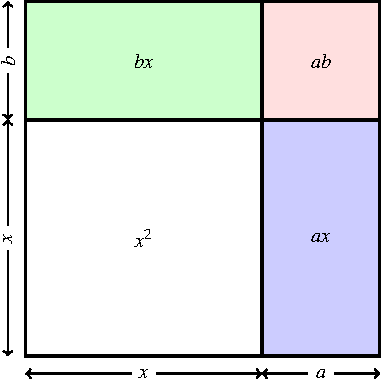
\includegraphics[scale=1]{image/08/quadratic-as-square.pdf}
\caption{%%
  The quadratic function $f(x) = (x + a)(x + b)$ can be interpreted as
  a rectangle whose base and height have lengths $x + a$ and $x + b$,
  respectively.
}
\label{fig:quadratic_as_rectangle}
\end{figure}

A quadratic function can be interpreted as the area of a rectangle.
Suppose you have the function
%%
\begin{equation}
\label{eqn:quadratic_function_rectangle}
f(x)
=
(x + a)(x + b)
\end{equation}
%%
where $x \geq 0$ is a real variable and the numbers $a \geq 0$ and
$b \geq 0$ are fixed constants.  You can interpret the factor
$x + a$ as the length of a rectangle.  Hence the factor $x + b$ can be
interpreted as the width of a rectangle.  This interpretation is
illustrated in \Figure{fig:quadratic_as_rectangle}.
Equation~\eqref{eqn:quadratic_function_rectangle} is indeed a
quadratic function because you can use the distributive laws to expand
the right-hand side to get
%%
\begin{equation}
\label{eqn:rectangle_as_quadratic}
\begin{aligned}
f(x)
&=
x(x + b) + a(x + b) \\[4pt]
&=
x^2 + bx + ax + ab \\[4pt]
&=
x^2 + (a + b)x + ab.
\end{aligned}
\end{equation}
%%
You can also prove \Equation{eqn:rectangle_as_quadratic} by using
geometry.

To prove the equation
\[
f(x)
=
(x + a)(x + b)
=
x^2 + (a + b)x + ab
\]
by geometry, note that if $a \geq 0$ and $b \geq 0$ then you have the
following cases:
%%
\begin{packedenumeral}
\item $a = 0$ and $b > 0$; or

\item $a > 0$ and $b = 0$; or

\item $a = b = 0$.
\end{packedenumeral}
%%
No matter what the values of $a$ and $b$ are, the function $f(x)$ can
be represented as the larger rectangle shown in
\Figure{fig:quadratic_as_rectangle}.  The larger rectangle has a
length and width of $x + a$ and $x + b$, respectively, and therefore
an area of $f(x) = (x + a)(x + b)$.  Note that the larger rectangle
can be divided into a number of smaller shapes: a smaller square and
three smaller rectangles.  The smaller square~(i.e.~the white square
in \Figure{fig:quadratic_as_rectangle}) has a side length of $x$, so
the square has an area of $x^2$.  The top rectangle~(i.e.~the green
rectangle in \Figure{fig:quadratic_as_rectangle}) has a length and
width of $x$ and $b$, respectively, so its area is $bx$.  The smaller
rectangle in the top-right corner~(i.e.~the pink rectangle in
\Figure{fig:quadratic_as_rectangle}) has a length and width of $a$ and
$b$, respectively, hence its area is $ab$.  The rectangle to the
right~(i.e.~the purple rectangle in
\Figure{fig:quadratic_as_rectangle}) has a length and width of $a$ and
$x$, respectively, thus an area of $ax$.  Adding together the area of
the four smaller shapes shows that the total area is
\[
x^2 + ax + bx + ab
=
x^2 + (a + b)x + ab.
\]
The four smaller shapes result from cutting the larger rectangle in
the way shown in \Figure{fig:quadratic_as_rectangle}.  In other words,
the total area of the four smaller shapes is the same as the area of
the larger rectangle.  Therefore you have proved that
\[
(x + a) (b + b)
=
x^2 + (a + b)x + ab.
\]


%%%%%%%%%%%%%%%%%%%%%%%%%%%%%%%%%%%%%%%%%%%%%%%%%%%%%%%%%%%%%%%%%%%%%%%%%%%

\section{Graphing}
\label{sec:graphing}

In the rest of this document, you will explore a number of ways to
sketch the graph of a quadratic function.  This section will show you
a graph drawing technique that works for any quadratic function.
Let's start with an example.

\begin{example}
Sketch a graph of the function $f(x) = x^2$.
\end{example}

\begin{solution}
Let's calculate the values of the function $f(x) = x^2$ for
$x = \quadruple{-3}{-2}{2}{3}$.  Note that you have
\[
f(2) = f(-2) = 4
%%
\qquad
\text{and}
\qquad
%%
f(3) = f(-3) = 9.
\]
Plot these points on one set of coordinate axes and draw a line
through the points to get the graph in \Figure{fig:quadratic_a_1}.
Note that $f(0) = 0$ so the graph of $f(x) = x^2$ touches the origin.
\end{solution}

The general shape of the graph of any quadratic function looks like
the beak of a duck~(or a nose).  The usual name for this graph is a
\emph{parabola}.  Note the tip or \emph{vertex} of the parabola.  The
vertex can be either the highest or lowest point of the parabola.

\begin{figure}[!htbp]
\centering
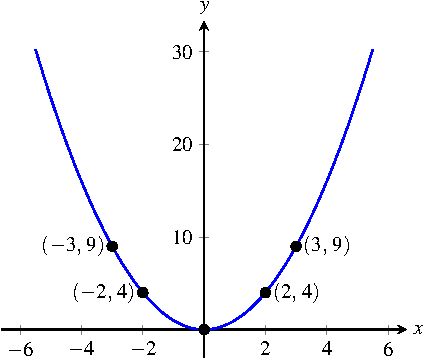
\includegraphics[scale=1.2]{image/08/a-1.pdf}
\caption{%%
  A graph of the function $f(x) = x^2$.  The general shape of the
  graph is called a \emph{parabola}.  The \emph{vertex} of the
  parabola is its highest or lowest point.  In this case, the vertex
  of $f(x) = x^2$ is the origin $\tuple{0}{0}$, which is the lowest
  point of the function.
}
\label{fig:quadratic_a_1}
\end{figure}

\begin{exercise}
For the quadratic function $f(x) = x^2$, verify that you have the
following equalities:
\[
f(2) = f(-2)
%%
\qquad
\text{and}
\qquad
%%
f(3) = f(-3).
\]
\end{exercise}
%%
\ifbool{showSolution}{
\begin{solution}
If $x = 2$ or $x = -2$, then you have
%%
\begin{align*}
f(2)
&=
2^2 \\[4pt]
&=
(-1)^2 2^2 \\[4pt]
&=
(-2)^2 \\[4pt]
&=
f(-2).
\end{align*}
%%
Finally, if $x = 3$ or $x = -3$ then you can write
%%
\begin{align*}
f(3)
&=
3^2 \\[4pt]
&=
(-1)^2 3^2 \\[4pt]
&=
(-3)^2 \\[4pt]
&=
f(-3).
\end{align*}
\end{solution}
}{}

Generally speaking, how would you draw the graph of
$f(x) = ax^2 + bx + c$?  A good strategy would be to start at the
vertex of the parabola and choose a few values of $x$ that are equally
spaced.  If the vertex of the parabola is $\tuple{\alpha}{\beta}$, the
following values of $x$
\[
\quintuple{\alpha-2}{\alpha-1}{\alpha}{\alpha+1}{\alpha+2}
\]
should usually be good enough for a rough sketch of the graph of
$f(x)$.  Of course, you still need to calculate the function values
$f(\alpha-2)$, $f(\alpha-1)$, $f(\alpha+1)$, and $f(\alpha+2)$.  Note
that the graph of the quadratic function $f(x)$ is symmetric about the
vertex $\tuple{\alpha}{\beta}$.
\Problem{prob:quadratic_symmetric_about_vertex} asks you to prove this
fact.  To say that $f(x)$ is symmetric about the vertex means that, in
particular, you have the equalities
\[
f(\alpha+1) = f(\alpha-1)
%%
\qquad
\text{and}
\qquad
%%
f(\alpha+2) = f(\alpha-2).
\]
Consequently, you need only to calculate two function values, not
four.  The above strategy is illustrated in
\Figure{fig:sketch_parabola}.

\begin{figure}[!htbp]
\centering
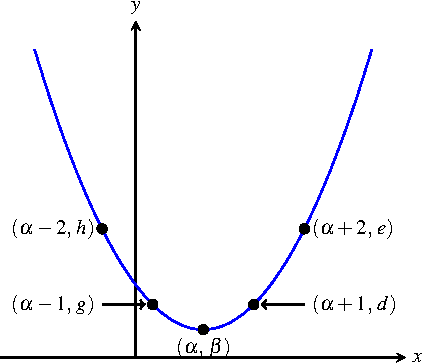
\includegraphics[scale=1.2]{image/08/a1-bminus4-c10.pdf}
\caption{%%
  Sketching the graph of a quadratic function.  First, locate the
  vertex $\tuple{\alpha}{\beta}$ of the function.  From there, spread
  outward with a few points.  Finally, you connect the dots.  Note
  that the graph is symmetric about the vertex.
}
\label{fig:sketch_parabola}
\end{figure}

The problem now is: How do you calculate the vertex of the parabola?
If you have a quadratic function of the form $f(x) = ax^2 + bx + c$,
the vertex~(i.e.~the highest or lower point) of the function is
located at the $x$-coordinate
%%
\begin{equation}
\label{eqn:parabola_tip_x_coordinate}
x
=
-\frac{b}{2a}.
\end{equation}
%%
Substitute \Expression{eqn:parabola_tip_x_coordinate} into the
function $f(x)$ to obtain the corresponding $y$-coordinate.  For now,
do not worry about how \Expression{eqn:parabola_tip_x_coordinate} was
derived.  This will be shown later on.

\begin{example}
\label{ex:quadratic_graph_a1_b1_c1}
Sketch a graph of the quadratic function $f(x) = x^2 + x + 1$.
\end{example}

\begin{solution}
The first thing you should do is determine the vertex of the parabola.
You have the values $a = 1$ and $b = 1$.  Use
\Expression{eqn:parabola_tip_x_coordinate} to see that the
$x$-coordinate of the vertex is
%%
\begin{align*}
x
&=
-\frac{1}{2 \times 1} \\[4pt]
&=
-\frac{1}{2}.
\end{align*}
%%
The $y$-coordinate of the vertex is
%%
\begin{align*}
y
&=
f(-1/2) \\[4pt]
&=
\parenthesis*{-\frac{1}{2}}^2 + \parenthesis*{-\frac{1}{2}} + 1 \\[4pt]
&=
\frac{1}{4} - \frac{1}{2} + 1 \\[4pt]
&=
\frac{1}{4} - \frac{2}{4} + \frac{4}{4} \\[4pt]
&=
\frac{1 - 2 + 4}{4} \\[4pt]
&=
\frac{3}{4}.
\end{align*}
%%
Thus the vertex of the parabola is the point
$\tuple{-\frac{1}{2}}{\frac{3}{4}}$.  Next, choose the $x$-coordinates
%%
\begin{equation}
\label{eqn:a1_b1_c1_x_coordinates}
\frac{1}{2} = -\frac{1}{2} + 1
%%
\qquad
\text{and}
\qquad
%%
\frac{3}{2} = -\frac{1}{2} + 2
\end{equation}
%%
whose corresponding $y$-coordinates are $\frac{7}{4}$ and
$\frac{19}{4}$, respectively.  These $y$-coordinates also correspond
to the $x$-coordinates
\[
-\frac{3}{2}
=
-\frac{1}{2} - 1
%%
\qquad
\text{and}
\qquad
%%
-\frac{5}{2}
=
-\frac{1}{2} - 2
\]
respectively.  Then you have
\[
f(1/2) = f(-3/2)
%%
\qquad
\text{and}
\qquad
%%
f(3/2) = f(-5/2).
\]
Plot the above five points, connect the dots, and you get the graph
in \Figure{fig:quadratic_graph_a1_b1_c1}.
\end{solution}

\begin{figure}[!htbp]
\centering
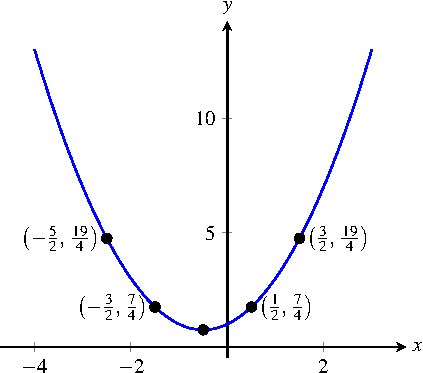
\includegraphics[scale=1.2]{image/08/a1-b1-c1.pdf}
\caption{%%
  A graph of the quadratic function $f(x) = x^2 + x + 1$.  The vertex
  of the function occurs at the point
  $\tuple{-\frac{1}{2}}{\frac{3}{4}}$.
}
\label{fig:quadratic_graph_a1_b1_c1}
\end{figure}

\begin{exercise}
For the $x$-coordinates~\eqref{eqn:a1_b1_c1_x_coordinates} in
\Example{ex:quadratic_graph_a1_b1_c1}, verify that the corresponding
$y$-coordinates are $\frac{7}{4}$ and $\frac{19}{4}$.
\end{exercise}
%%
\ifbool{showSolution}{
\begin{solution}
The quadratic function is $f(x) = x^2 + x + 1$.  For $x = 1/2$ you have
%%
\begin{align*}
f(1/2)
&=
\parenthesis*{\frac{1}{2}}^2 + \frac{1}{2} + 1 \\[4pt]
&=
\frac{1}{4} + \frac{1}{2} + 1 \\[4pt]
&=
\frac{1}{4} + \frac{2}{4} + \frac{4}{4} \\[4pt]
&=
\frac{7}{4}.
\end{align*}
%%
Finally, for $x = 3/2$ you have
%%
\begin{align*}
f(3/2)
&=
\parenthesis*{\frac{3}{2}}^2 + \frac{3}{2} + 1 \\[4pt]
&=
\frac{9}{4} + \frac{3}{2} + 1 \\[4pt]
&=
\frac{9}{4} + \frac{6}{4} + \frac{4}{4} \\[4pt]
&=
\frac{19}{4}.
\end{align*}
\end{solution}
}{}

\begin{exercise}
Sketch a graph of the function $f(x) = x^2 - 2x + 2$.
\end{exercise}
%%
\ifbool{showSolution}{
\begin{solution}
First, you determine the vertex of the function $f(x)$.  You have
$a = 1$ and $b = -2$.  Use \Expression{eqn:parabola_tip_x_coordinate}
to see that the $x$-coordinate of the vertex is
%%
\begin{align*}
x
&=
-\frac{-2}{2 \times 1} \\[4pt]
&=
\frac{2}{2} \\[4pt]
&=
1.
\end{align*}
%%
The $y$-coordinate of the vertex is
%%
\begin{align*}
f(1)
&=
1^2 - 2(1) + 2 \\[4pt]
&=
1 - 2 + 2 \\[4pt]
&=
1.
\end{align*}
%%
Hence the vertex of the function $f(x)$ is the point $\tuple{1}{1}$.
Next, choose the following values for $x$:
\[
2 = 1 + 1
%%
\qquad
\text{and}
\qquad
%%
3 = 1 + 2.
\]
The corresponding function values are
\[
f(2) = f(0) = 2
%%
\qquad
\text{and}
\qquad
%%
f(3) = f(-1) = 5.
\]
Plot the above five points~(including the vertex) to obtain the graph
shown in \Figure{fig:graph_a1_bminus2_c2}.

\begin{figure}[!htbp]
\centering
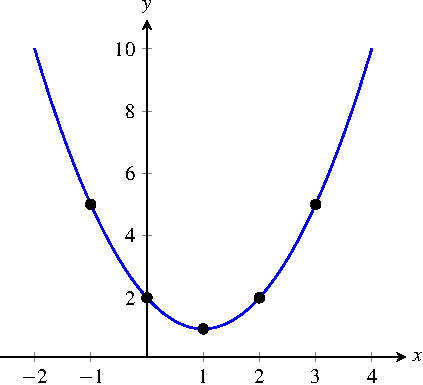
\includegraphics[scale=1.2]{image/08/a1-bminus2-c2.pdf}
\caption{%%
  A graph of the function $f(x) = x^2 - 2x + 2$.  The vertex of the
  function occurs at the point $\tuple{1}{1}$.
}
\label{fig:graph_a1_bminus2_c2}
\end{figure}
\end{solution}
}{}


%%%%%%%%%%%%%%%%%%%%%%%%%%%%%%%%%%%%%%%%%%%%%%%%%%%%%%%%%%%%%%%%%%%%%%%%%%%

\section{Quadratic formula}
\label{sec:quadratic_formula}

This section will show you another way to draw a graph of a quadratic
function.  The graph sketching technique uses the
\emph{quadratic formula}.  Given a quadratic function
$f(x) = ax^2 + bx + c$, sometimes a problem requires you to determine
the values of $x$ such that $f(x) = 0$.  Those values of $x$ for which
the equation $f(x) = 0$ is true are called the \emph{roots} of
$f(x)$.  The roots of $f(x)$ are also the points where the graph of
$f(x)$ intersects the $x$-axis.  Thus the roots of $f(x)$ are also the
$x$-intercepts of $f(x)$.  When you need to calculate the roots of
$f(x)$, the quadratic formula is guaranteed to provide you with at
least one root.  But what is the quadratic formula?  How is it
derived?  And how can the quadratic formula be used to sketch a graph
of a quadratic function?

\begin{exercise}
\label{ex:completing_the_square}
Let $\pair{a}{b} \in \RR$ be constants such that $a \neq 0$ and let
$x$ be a real variable.  Show that
\[
\parenthesis*{x + \frac{b}{2a}}^2
=
x^2 + \frac{b}{a} x + \parenthesis*{\frac{b}{2a}}^2.
\]
\end{exercise}
%%
\ifbool{showSolution}{
\begin{solution}
Use the distributive laws to expand
$\parenthesis*{x + \frac{b}{2a}}^2$ and you get
%%
\begin{align*}
\parenthesis*{x + \frac{b}{2a}}^2
&=
\parenthesis*{x + \frac{b}{2a}} \parenthesis*{x + \frac{b}{2a}} \\[4pt]
&=
x \parenthesis*{x + \frac{b}{2a}}
+
\frac{b}{2a} \parenthesis*{x + \frac{b}{2a}} \\[4pt]
&=
x^2 + \frac{b}{2a} x + \frac{b}{2a} x + \parenthesis*{\frac{b}{2a}}^2 \\[4pt]
&=
x^2 + 2 \times \frac{b}{2a} x + \parenthesis*{\frac{b}{2a}}^2 \\[4pt]
&=
x^2 + \frac{b}{a} x + \parenthesis*{\frac{b}{2a}}^2
\end{align*}
%%
as required.
\end{solution}
}{}

\begin{exercise}
\label{ex:completing_the_square_redux}
Let $x$ be a real variable and suppose $\triple{a}{b}{c} \in \RR$ are
constants such that $a \neq 0$.  Show that the expression
\[
\parenthesis*{
  x + \frac{b}{2a}
}^2
=
\frac{
  b^2 - 4ac
}{
  4a^2
}
\]
can also be written as $(2ax + b)^2 = b^2 - 4ac$.  Given any quadratic
function $f(x)$, the above method of writing the equation $f(x) = 0$
is called \emph{completing the square}.
\end{exercise}
%%
\ifbool{showSolution}{
\begin{solution}
The statement of the problem assumes that the expression
\[
\parenthesis*{
  x + \frac{b}{2a}
}^2
=
\frac{
  b^2 - 4ac
}{
  4a^2
}
\]
is true.  For the sake of argument, you can assume that the expression
is true.  Multiplying both sides by $4a^2$ produces the expression
%%
\begin{equation}
\label{eqn:complete_the_square_no_denominator}
4a^2 \parenthesis*{x + \frac{b}{2a}}^2
=
b^2 - 4ac
\end{equation}
%%
where the left-hand side can be factored as
%%
\begin{equation}
\label{eqn:complete_the_square_factored}
\begin{aligned}
4a^2 \parenthesis*{x + \frac{b}{2a}}^2
&=
(2a)^2 \parenthesis*{x + \frac{b}{2a}}^2 \\[4pt]
&=
\squarebracket*{2a \parenthesis*{x + \frac{b}{2a}}}^2 \\[4pt]
&=
\parenthesis*{2ax + 2a \times \frac{b}{2a}}^2 \\[4pt]
&=
\parenthesis*{2ax + b}^2.
\end{aligned}
\end{equation}
%%
Conclude from
\Expressions{eqn:complete_the_square_no_denominator}{eqn:complete_the_square_factored}
that $(2ax + b)^2 = b^2 - 4ac$.
\end{solution}
}{}

\begin{exercise}
Let $a \in \RR$ and consider the numbers $\pm\sqrt{a}$.  Here the
symbol ``$\pm$'' means that you have both of $\sqrt{a}$ and
$-\sqrt{a}$.  If $x = \pm\sqrt{a}$, prove that $x^2 = a$.
\end{exercise}
%%
\ifbool{showSolution}{
\begin{solution}
You must prove two statements:
%%
\begin{packedenumeral}
\item\label{case:x_sqrt_a_implies_x_squared_a}
  If $x = \sqrt{a}$ then $x^2 = a$.

\item\label{case:x_minus_sqrt_a_implies_x_squared_a}
  If $x = -\sqrt{a}$ then $x^2 = a$.
\end{packedenumeral}
%%
First, let's prove \Statement{case:x_sqrt_a_implies_x_squared_a}.  If
$x = \sqrt{a}$, then you can square both sides of the equation to get
$x^2 = (\sqrt{a})^2$.  Since $\sqrt{a} = a^{1/2}$, then you can write
the expression $x^2 = (\sqrt{a})^2$ as
%%
\begin{equation}
\label{eqn:x_sqrt_a_implies_x_squared_a}
\begin{aligned}
x^2
&=
(\sqrt{a})^2 \\[4pt]
&=
(a^{1/2})^2 \\[4pt]
&=
a^{2/2} \\[4pt]
&=
a.
\end{aligned}
\end{equation}
%%
Finally, let's prove
\Statement{case:x_minus_sqrt_a_implies_x_squared_a}.  If
$x = -\sqrt{a}$, then squaring both sides of the equation results in
%%
\begin{align*}
x^2
&=
\bigparen{(-1)\sqrt{a}}^2 \\[4pt]
&=
(-1)^2 (\sqrt{a})^2 \\[4pt]
&=
(\sqrt{a})^2.
\end{align*}
%%
The latter equation can be simplied to $x^2 = a$ by using
\Expression{eqn:x_sqrt_a_implies_x_squared_a}.  Therefore if
$x = \pm\sqrt{a}$ then you have $x^2 = a$.
\end{solution}
}{}

\begin{exercise}
\label{ex:x_squared_a_implies_plus_minus_sqrt_a}
If $a$ is a real number such that $x^2 = a$, prove that
$x = \pm\sqrt{a}$.
\end{exercise}
%%
\ifbool{showSolution}{
\begin{solution}
You have two statements to prove:
%%
\begin{packedenumeral}
\item\label{case:x_squared_a_sqrt_a}
  If $a \in \RR$ such that $x^2 = a$, then $x = \sqrt{a}$.

\item\label{case:x_squared_a_minus_sqrt_a}
  If $a \in \RR$ such that $x^2 = a$, then $x = -\sqrt{a}$.
\end{packedenumeral}
%%
First, let's prove \Statement{case:x_squared_a_sqrt_a}.  You know that
$x^2 = a$ and the square root of any number $c \in \RR$ can be written
as $\sqrt{c} = c^{1/2}$.  Taking the square root of both sides of the
equation $x^2 = a$ and you get $(x^2)^{1/2} = a^{1/2}$, which can also
be written as $x^{2/2} = a^{1/2}$.  The latter equation simplifies to
$x = \sqrt{a}$ because $x^{2/2} = x^1 = x$.

Finally, let's prove \Statement{case:x_squared_a_minus_sqrt_a}.  You
know that $x^2 = a$ and since $a = (-1)^2 a$, you can also write
$x^2 = (-1)^2 a$.  Take the square root of both sides of the last
equation to get $(x^2)^{1/2} = \bigparen{(-1)^2 a}^{1/2}$, which can
be written as $x^{2/2} = (-1)^{2/2} a^{1/2}$.  Use the fact that
$(-1)^{2/2} = (-1)^1 = -1$ to write $x = -\sqrt{a}$.
\end{solution}
}{}

First, let's derive the quadratic formula.  When you write $f(x) = 0$,
it is the same as writing $ax^2 + bx + c = 0$.  When you require a
value of $x$ such that $f(x) = 0$, i.e.~a root of $f(x)$, what you
really want is to solve the equation $ax^2 + bx + c = 0$ for $x$.  In
the last equation, dividing each term by $a$ results in the equivalent
expression
\[
x^2 + \frac{b}{a} x + \frac{c}{a}
=
0.
\]
Now move the term $c/a$ to the right-hand side to obtain
%%
\begin{equation}
\label{eqn:quadratic_formula_factor_LHS}
x^2 + \frac{b}{a} x
=
-\frac{c}{a}.
\end{equation}
%%
The problem now is to factor the left-hand side of
\Equation{eqn:quadratic_formula_factor_LHS}.  From
\Exercise{ex:completing_the_square} you know that the square
$\parenthesis*{x + \frac{b}{2a}}^2$ can be expanded to become
\[
\parenthesis*{x + \frac{b}{2a}}^2
=
x^2 + \frac{b}{a} x + \parenthesis*{\frac{b}{2a}}^2
\]
where the expression $x^2 + \frac{b}{a} x$ is the same as the
left-hand side of \Equation{eqn:quadratic_formula_factor_LHS}.  Adding
$\parenthesis*{\frac{b}{2a}}^2$ to both sides of
\Equation{eqn:quadratic_formula_factor_LHS} results in
%%
\begin{align*}
x^2 + \frac{b}{a} x + \parenthesis*{\frac{b}{2a}}^2
&=
-\frac{c}{a} + \parenthesis*{\frac{b}{2a}}^2 \\[4pt]
&=
-\frac{c}{a} + \frac{b^2}{4a^2} \\[4pt]
&=
-\frac{c}{a} \times \frac{4a}{4a} + \frac{b^2}{4a^2} \\[4pt]
&=
-\frac{4ac}{4a^2} + \frac{b^2}{4a^2} \\[4pt]
&=
\frac{
  b^2 - 4ac
}{
  4a^2
}.
\end{align*}
%%
Now use \Exercise{ex:completing_the_square} to factor the left-hand
side of the latter expression and you can write
\Equation{eqn:quadratic_formula_factor_LHS} as
\[
\parenthesis*{x + \frac{b}{2a}}^2
=
\frac{
  b^2 - 4ac
}{
  4a^2
}.
\]
By \Exercise{ex:completing_the_square_redux} this expression is the
same as the equation $(2ax + b)^2 = b^2 - 4ac$.  Use
\Exercise{ex:x_squared_a_implies_plus_minus_sqrt_a} to write the last
equation as $2ax + b = \pm\sqrt{b^2 - 4ac}$.  Solve for $x$ and you
obtain
%%
\begin{align*}
x
&=
\frac{
  -b \pm \sqrt{b^2 - 4ac}
}{
  2a
}
\end{align*}
%%
which is called the \emph{quadratic formula}.  The above can be
summarised as follows.

\begin{theorem}
\label{thm:quadratic_formula}
\textbf{Quadratic formula.}
Let $\triple{a}{b}{c} \in \RR$ such that $a \neq 0$ and consider the
quadratic function $f(x) = ax^2 + bx + c$.  The roots of $f(x)$ can be
written as
%%
\begin{equation}
\label{eqn:quadratic_formula}
x
=
\frac{
  -b \pm \sqrt{b^2 - 4ac}
}{
  2a
}.
\end{equation}
\end{theorem}

What does the quadratic \Formula{eqn:quadratic_formula} mean?  How do
you make sense of the equation?  Let's assume you have a quadratic
function $f(x) = ax^2 + bx + c$ with $\triple{a}{b}{c}$ being real
numbers such that $a \neq 0$.
Expression~\eqref{eqn:quadratic_formula} states that there are values
of $x$ such that $f(x) = 0$ and those values of $x$ can be written as
\[
x
=
\frac{
  -b + \sqrt{b^2 - 4ac}
}{
  2a
}
%%
\qquad
\text{and}
\qquad
%%
x
=
\frac{
  -b - \sqrt{b^2 - 4ac}
}{
  2a
}.
\]
How can you use the quadratic formula to help you sketch a graph of a
quadratic function?  In the graph of $f(x)$, the $x$-intercept or root
of $f(x)$ is obtained by setting $f(x) = 0$ and solving the last
equation for $x$.  The whole point of \Theorem{thm:quadratic_formula}
is to help you calculate the $x$-intercepts of a quadratic function.
\Theorem{thm:quadratic_formula} also says that a quadratic function
has at most two $x$-intercepts.  You also know
from \Section{sec:graphing} that the vertex of $f(x)$ occurs at
the $x$-coordinate given by \Equation{eqn:parabola_tip_x_coordinate}.
To sketch a graph of $f(x)$, you first calculate the vertex and roots
of $f(x)$.  You then plot the three points on one set of coordinate
axes and connect the dots to obtain a graph of $f(x)$.  The next
example should help to clarify the theory.

\begin{example}
Sketch a graph of the function $f(x) = x^2 - x - 2$.
\end{example}

\begin{solution}
You have the values $a = 1$, $b = -1$, and $c = -2$.  You can use
three points to draw a graph of $f(x)$.  The first point is the
vertex of the parabola.  The other two points are the $x$-intercepts
of $f(x)$.

First, let's determine the vertex of $f(x)$.  From
\Equation{eqn:parabola_tip_x_coordinate} you know that the vertex of
the parabola occurs at the $x$-coordinate
%%
\begin{align*}
x
&=
-\frac{-1}{2 \times 1} \\[4pt]
&=
\frac{1}{2}.
\end{align*}
%%
Then the $y$-coordinate of the vertex is
%%
\begin{align*}
y
&=
f(1/2) \\[4pt]
&=
\parenthesis*{\frac{1}{2}}^2 - \frac{1}{2} - 2 \\[4pt]
&=
\frac{1}{4} - \frac{2}{4} - \frac{8}{4} \\[4pt]
&=
\frac{1 - 2 - 8}{4} \\[4pt]
&=
-\frac{9}{4}.
\end{align*}
%%
Thus the quadratic function $f(x)$ has its vertex at the point
$\tuple{\frac{1}{2}}{-\frac{9}{4}}$.

Next, let's calculate the $x$-intercepts~(or roots) of $f(x)$.  From
\Equation{eqn:quadratic_formula} you know that one of the
$x$-intercepts occurs at
%%
\begin{align*}
x
&=
\frac{
  -(-1) + \sqrt{(-1)^2 - 4(1)(-2)}
}{
  2(1)
} \\[4pt]
&=
\frac{
  1 + \sqrt{1 + 8}
}{
  2
} \\[4pt]
&=
\frac{
  1 + \sqrt{9}
}{
  2
} \\[4pt]
&=
\frac{
  1 + 3
}{
  2
} \\[4pt]
&=
2.
\end{align*}
%%
The other $x$-intercept occurs at
%%
\begin{align*}
x
&=
\frac{
  -(-1) - \sqrt{(-1)^2 - 4(1)(-2)}
}{
  2(1)
} \\[4pt]
&=
\frac{
  1 - \sqrt{9}
}{
  2
} \\[4pt]
&=
\frac{
  1 - 3
}{
  2
} \\[4pt]
&=
-1.
\end{align*}
%%
In other words, you have two different $x$-intercepts that occur at
the points $\tuple{2}{0}$ and $\tuple{-1}{0}$.  Plot the vertex and
the two $x$-intercepts on one set of coordinate axes, draw a line
through the points, and you obtain the graph in
\Figure{fig:a1_bminus1_cminus2}.
\end{solution}

\begin{figure}[!htbp]
\centering
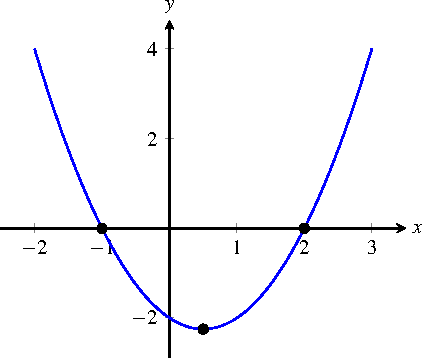
\includegraphics[scale=1]{image/08/a1-bminus1-cminus2.pdf}
\caption{%%
  Graph of the function $f(x) = x^2 - x - 2$ through three points.
  The three points are the vertex and roots of $f(x)$.  In this case,
  the vertex of $f(x)$ is also the lowest point in the graph of
  $f(x)$.
}
\label{fig:a1_bminus1_cminus2}
\end{figure}

\begin{exercise}
Use the quadratic formula to sketch the graph of
\[
f(x)
=
-2x^2 + x + 3.
\]
\end{exercise}
%%
\ifbool{showSolution}{
\begin{solution}
You have the values $a = -2$, $b = 1$, and $c = 3$.  You can draw the
graph of $f(x) = -2x^2 + x + 3$ by using three points: the vertex and
the two $x$-intercepts of $f(x)$.

First, let's calculate the vertex of $f(x)$.  Use
\Equation{eqn:parabola_tip_x_coordinate} to see that the vertex occurs
at the $x$-coordinate
%%
\begin{align*}
x
&=
-\frac{1}{2(-2)} \\[4pt]
&=
\frac{1}{4}.
\end{align*}
%%
The $y$-coordinate of the vertex is
%%
\begin{align*}
y
&=
f(1/4) \\[4pt]
&=
-2\parenthesis*{\frac{1}{4}}^2 + \frac{1}{4} + 3 \\[4pt]
&=
-2 \times \frac{1}{16} + \frac{4}{16} + 3 \\[4pt]
&=
\frac{4 - 2}{16} + 3 \\[4pt]
&=
\frac{1}{8} + 3 \\[4pt]
&=
\frac{1}{8} + \frac{24}{8} \\[4pt]
&=
\frac{25}{8}.
\end{align*}
%%
Thus $f(x)$ has its vertex at the point
$\tuple{\frac{1}{4}}{\frac{25}{8}}$.

Next, you calculate the $x$-intercepts~(which are also the roots) of
$f(x)$.  Using the quadratic \Formula{eqn:quadratic_formula}, you see
that an $x$-intercept has the $x$-coordinate
%%
\begin{align*}
x
&=
\frac{
  -1 + \sqrt{1^2 - 4(-2)(3)}
}{
  2(-2)
} \\[4pt]
&=
\frac{
  -1 + \sqrt{1 + 24}
}{
  -4
} \\[4pt]
&=
\frac{
  -1 + 5
}{
  -4
} \\[4pt]
&=
-1.
\end{align*}
%%
The other $x$-intercept has the $x$-coordinate
%%
\begin{align*}
x
&=
\frac{
  -1 - \sqrt{1^2 - 4(-2)(3)}
}{
  2(-2)
} \\[4pt]
&=
\frac{
  -1 - 5
}{
  -4
} \\[4pt]
&=
\frac{-6}{-4} \\[4pt]
&=
\frac{3}{2}.
\end{align*}
%%
You now have the $x$-intercepts $\tuple{-1}{0}$ and
$\tuple{\frac{3}{2}}{0}$.

Finally, you plot the above three points on one set of coordinate
axes.  Draw a line through the points and you get the graph in
\Figure{fig:aminus2_b1_c3}.

\begin{figure}[!htbp]
\centering
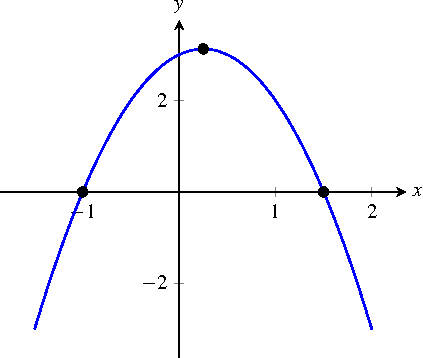
\includegraphics[scale=1]{image/08/aminus2-b1-c3.pdf}
\caption{%%
  Graph of the function $f(x) = -2x^2 + x + 3$ through three points.
  The three points are the vertex $\tuple{\frac{1}{4}}{\frac{25}{8}}$
  and the roots $\tuple{-1}{0}$ and $\tuple{\frac{3}{2}}{0}$ of
  $f(x)$.  In this case, the vertex of $f(x)$ is the highest point in
  the graph of $f(x)$.
}
\label{fig:aminus2_b1_c3}
\end{figure}
\end{solution}
}{}

\begin{exercise}
Use the quadratic formula to sketch the graph of $f(x) = -x^2 + 1$.
\end{exercise}

\ifbool{showSolution}{
\begin{solution}
You have the values $a = -1$ and $c = 1$.  The value of $b$ is
$b = 0$ because $f(x) = -x^2 + 1 = -x^2 + 0x + 1$.  Again, you can use
three points to draw the graph of $f(x)$.  Those three points are the
vertex and $x$-intercepts of $f(x)$.  The $x$-intercepts of $f(x)$ are
also called the roots of $f(x)$.

First, you calculate the vertex of $f(x)$.  Use
\Equation{eqn:parabola_tip_x_coordinate} to see that the vertex of
$f(x)$ occurs at the $x$-coordinate
\[
x
=
-\frac{0}{2(-1)}
=
0
\]
whose corresponding $y$-coordinate is
\[
y
=
f(0)
=
-0^2 + 1
=
1.
\]
The function $f(x)$ has its vertex at the point $\tuple{0}{1}$.

Next, you calculate the roots of $f(x)$.  Use
\Equation{eqn:quadratic_formula} to obtain the root
%%
\begin{align*}
x
&=
\frac{
  -0 + \sqrt{0^2 - 4(-1)(1)}
}{
  2(-1)
} \\[4pt]
&=
\frac{
  \sqrt{4}
}{
  -2
} \\[4pt]
&=
-1.
\end{align*}
%%
The other root of $f(x)$ occurs at
%%
\begin{align*}
x
&=
\frac{
  -0 - \sqrt{0^2 - 4(-1)(1)}
}{
  2(-1)
} \\[4pt]
&=
\frac{
  -\sqrt{4}
}{
  -2
} \\[4pt]
&=
1.
\end{align*}
%%
Thus $f(x)$ has its $x$-intercepts at the points $\tuple{-1}{0}$ and
$\tuple{1}{0}$.  Finally, you plot the three points and connect the
dots to obtain the graph in \Figure{fig:aminus1_c1}.
\end{solution}

\begin{figure}[!htbp]
\centering
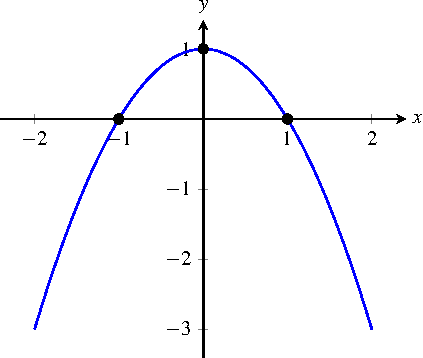
\includegraphics[scale=1]{image/08/aminus1-c1.pdf}
\caption{%%
  Graph of the function $f(x) = -x^2 + 1$ through three points.  The
  three points are the vertex $\tuple{0}{1}$ and the $x$-intercepts
  $\tuple{-1}{0}$ and $\tuple{1}{0}$.  Note that in this case, the
  vertex of $f(x)$ is the highest point in the graph of $f(x)$.
}
\label{fig:aminus1_c1}
\end{figure}
}{}


%%%%%%%%%%%%%%%%%%%%%%%%%%%%%%%%%%%%%%%%%%%%%%%%%%%%%%%%%%%%%%%%%%%%%%%%%%%

\section{The discriminant}

You have seen in \Section{sec:quadratic_formula} how the quadratic
formula can help you to sketch the graph of a quadratic function
$f(x)$.  The general strategy was to determine the vertex of $f(x)$
and then use the quadratic formula to calculate two $x$-intercepts of
$f(x)$.  You plot the three points on one set of coordinate axes and
connect the dots to obtain the graph of the function $f(x)$.  But this
strategy does not always work.

To understand why the graph drawing strategy
from \Section{sec:quadratic_formula} can fail, let's consider the
example of the function $f(x) = x^2$.  According to the strategy
from \Section{sec:quadratic_formula}, you first need to calculate the
vertex of $f(x)$.  This is easy.  You have the values $a = 1$ and
$b = c = 0$.  Just use \Equation{eqn:parabola_tip_x_coordinate} to see
that the $x$-coordinate of the vertex is
%%
\begin{align*}
x
&=
-\frac{0}{2(1)} \\[4pt]
&=
0.
\end{align*}
%%
The corresponding $y$-coordinate is
%%
\begin{align*}
y
&=
f(0) \\[4pt]
&=
0^2 \\[4pt]
&=
0.
\end{align*}
%%
Therefore the function $f(x) = x^2$ has its vertex at the origin.  Now
use the quadratic \Formula{eqn:quadratic_formula} to see that the
$x$-intercepts of $f(x)$ occur at the $x$-coordinate
%%
\begin{align*}
x
&=
\frac{
  -0 \pm \sqrt{0^2 - 4(1)(0)}
}{
  2(1)
} \\[4pt]
&=
\pm
\frac{
  \sqrt{0}
}{
  2
} \\[4pt]
&=
0
\end{align*}
%%
with the corresponding $y$-coordinate being $y = f(0) = 0$.  The
upshot is that the vertex of $f(x)$ is also its $x$-intercept,
i.e.~the point $\tuple{0}{0}$.  The strategy
from \Section{sec:quadratic_formula} for graphing a quadratic function
results in only one point, not the three that you require.  In the
case of the function $f(x) = x^2$, you should have used the strategy
from \Section{sec:graphing}.

\begin{exercise}
Consider the function $f(x) = x^2 + 2x + 1$.  Explain why the graph
drawing strategy from \Section{sec:quadratic_formula} cannot help you
with sketching the graph of $f(x)$.
\end{exercise}
%%
\ifbool{showSolution}{
\begin{solution}
First, let's calculate the vertex of $f(x)$.  From
\Equation{eqn:parabola_tip_x_coordinate}, the $x$-coordinate of the
vertex is
%%
\begin{align*}
x
&=
-\frac{2}{2(1)} \\[4pt]
&=
-1.
\end{align*}
%%
The corresponding $y$-coordinate is $y = f(-1) = 0$.  That is, the
vertex of $f(x)$ is located at the point $\tuple{-1}{0}$.

Next, you use the quadratic \Formula{thm:quadratic_formula} to
determine the $x$-intercepts of $f(x)$.  The $x$-coordinates of the
$x$-intercept are
%%
\begin{align*}
x
&=
\frac{
  -2 \pm \sqrt{2^2 - 4(1)(1)}
}{
  2(1)
} \\[4pt]
&=
\frac{
  -2 \pm \sqrt{4 - 4}
}{
  2
} \\[4pt]
&=
\frac{-2}{2} \\[4pt]
&=
-1.
\end{align*}
%%
The corresponding $y$-coordinate is $y = f(-1) = 0$.  In other words,
the function $f(x)$ has its $x$-intercepts at the point
$\tuple{-1}{0}$, which is also the vertex of $f(x)$.  In the case of
$f(x)$, the graph sketching strategy
from \Section{sec:quadratic_formula} results in only one point, not
the three that you need to draw the graph.
\end{solution}
}{}

Is there a way to determine when to use the strategies
from \Sections{sec:graphing}{sec:quadratic_formula} for graphing a
quadratic function?  The answer is yes, but you need to understand a
number called the \emph{discriminant} of a quadratic function.

\begin{definition}
\label{def:discriminant}
\textbf{Discriminant.}
Let $\triple{a}{b}{c} \in \RR$ such that $a \neq 0$ and consider the
quadratic function $f(x) = ax^2 + bx + c$.  If the roots of $f(x)$ are
\[
x
=
\frac{
  -b \pm \sqrt{b^2 - 4ac}
}{
  2a
}
\]
then the number $\Delta = b^2 - 4ac$ is called the \emph{discriminant}
of $f(x)$.
\end{definition}

Like any real number, the discriminant can take on one of three types
of values.  The discriminant can be either negative, zero, or
positive.  Depending on the value of the discriminant, a quadratic
function will have either zero, one, or two $x$-intercepts.  Let's
consider each of the three cases separately.  Suppose $f(x)$ is a
quadratic function whose discriminant is $\Delta$.

\begin{packedenumeral}
\item If $\Delta < 0$, then $f(x)$ does not intersect the $x$-axis.
  The graph of $f(x)$ lies wholly above or below the $x$-axis.  See
  \Figure{fig:negative_discriminant}.

\item If $\Delta = 0$, then $f(x)$ intersects the $x$-axis once.  The
  point of intersection is also the vertex of the quadratic function.
  This case is illustrated in \Figure{fig:zero_discriminant}.

\item If $\Delta > 0$, then $f(x)$ has two different $x$-intercepts.
  See \Figure{fig:positive_discriminant}.
\end{packedenumeral}

\begin{figure}[!htbp]
\centering
\subfigure[]{
  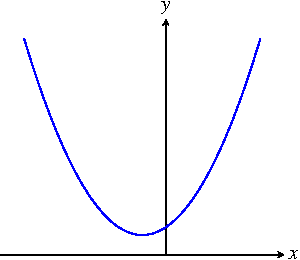
\includegraphics[scale=0.85]{image/08/a2-b1-c1.pdf}
}
%%
\quad
%%
\subfigure[]{
  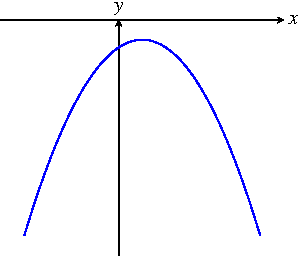
\includegraphics[scale=0.93]{image/08/aminus2-b1-cminus2.pdf}
}
\caption{%%
  When the discriminant is negative, the graph of a quadratic function
  does not intersect the $x$-axis.
}
\label{fig:negative_discriminant}
\end{figure}

\begin{figure}[!htbp]
\centering
\subfigure[]{
  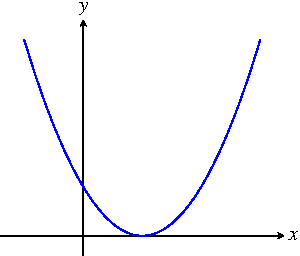
\includegraphics[scale=1]{image/08/a1-bminus2-c1.pdf}
}
%%
\qquad
%%
\subfigure[]{
  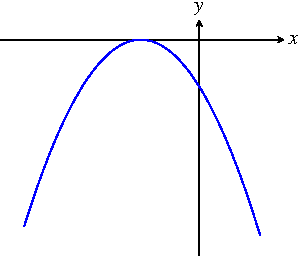
\includegraphics[scale=1]{image/08/aminus9quarter-bminus3-cminus1.pdf}
}
\caption{%%
  When the discriminant is zero, the graph of a quadratic function
  intersects the $x$-axis at exactly one point.
}
\label{fig:zero_discriminant}
\end{figure}

\begin{figure}[!htbp]
\centering
\subfigure[]{
  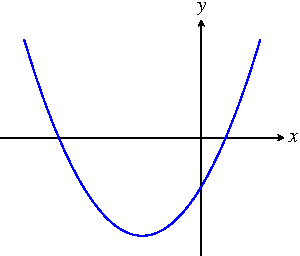
\includegraphics[scale=1]{image/08/a1-b2-cminus1.pdf}
}
%%
\qquad
%%
\subfigure[]{
  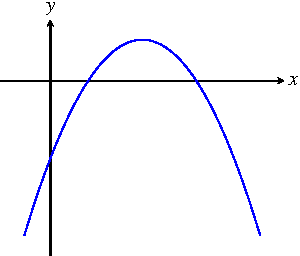
\includegraphics[scale=1]{image/08/aminus1-b3half-cminus2.pdf}
}
\caption{%%
  When the discriminant is positive, the graph of a quadratic function
  intersects the $x$-axis at two different points.
}
\label{fig:positive_discriminant}
\end{figure}

What all this means is that if the discriminant of a quadratic
function $f(x)$ is either negative or zero, then you should use the
strategy from \Section{sec:graphing} to sketch the graph of
$f(x)$.  If the discriminant of $f(x)$ is positive, then the strategy
from \Section{sec:quadratic_formula} can be used to draw the graph of
$f(x)$.  Or you could forget about \Section{sec:quadratic_formula}
entirely and use the technique from \Section{sec:graphing} because
the graph drawing strategy from that section will always work for any
quadratic function.  So why would you bother to learn about the
discriminant?

An answer can be found in
\Problems{prob:zero_discriminant}{prob:positive_discriminant} and can
be summarised as follows.  The discriminant of a quadratic function
$f(x)$ tells you how many roots $f(x)$ has.  The discriminant also
tells you how many times the graph of $f(x)$ will intersect the
$x$-axis.  You do not need to use the quadratic
\Formula{eqn:quadratic_formula} to know that $f(x)$ has either a
unique root or two different roots or that the graph of $f(x)$ does
not intersect the $x$-axis.  All you need to do is calculate the
discriminant of $f(x)$, which is much simpler to do than calculating
the actual roots of $f(x)$.

\begin{example}
Explain why the quadratic function $f(x) = 2x^2 + x + 1$ does not
intersect the $x$-axis.
\end{example}

\begin{solution}
The discriminant of $f(x)$ is
$\Delta = 1^2 - 4(2)(1) = 1 - 8 = -7$.  Since $\Delta$ is negative,
the graph of $f(x)$ does not intersect the $x$-axis.
\end{solution}

\begin{exercise}
How many different roots does the function $f(x) = x^2 - 2x + 1$ have?
How many times does the graph of $f(x)$ intersect the $x$-axis?
\end{exercise}
%%
\ifbool{showSolution}{
\begin{solution}
The discriminant of $f(x)$ is
$\Delta = (-2)^2 - 4(1)(1) = 4 - 4 = 0$.  Therefore $f(x)$ has a
unique root.  The graph of $f(x)$ will intersect the $x$-axis once
because the root of $f(x)$ lies on the $x$-axis.
\end{solution}
}{}

\begin{exercise}
Explain why $f(x) = -x^2 - \frac{7}{2}x - 2$ has two different roots.
How many times does the graph of $f(x)$ intersect the $x$-axis?
\end{exercise}
%%
\ifbool{showSolution}{
\begin{solution}
The discriminant of $f(x)$ is
$\Delta
=
\parenthesis*{-\frac{7}{2}}^2 - 4(-1)(-2)
=
\frac{49}{4} - 8$,
which is a positive number because $\Delta = 17/4$.  Therefore $f(x)$
has two different roots.  Since the roots of $f(x)$ are located on the
$x$-axis, it follows that the graph of $f(x)$ will intersect the
$x$-axis exactly twice.
\end{solution}
}{}


\newpage
%%%%%%%%%%%%%%%%%%%%%%%%%%%%%%%%%%%%%%%%%%%%%%%%%%%%%%%%%%%%%%%%%%%%%%%%%%%

\section*{Problem}

\begin{problem}
\item Read the following articles:

  \begin{packeditem}
  \item \emph{101 uses of a quadratic equation}

  \item \emph{101 uses of a quadratic equation: Part II}
  \end{packeditem}

  Try to understand as much as you can about how the quadratic
  functions are used.

\item\label{prob:zero_discriminant}
  Let $f(x)$ be a quadratic function whose discriminant is zero.
  %%
  \begin{packedenum}
  \item\label{subprob:zero_discriminant_unique_root}
    Prove that all the roots of $f(x)$ occur at the same value of
    $x$.

  \item\label{subprob:zero_discriminant_root_is_tip_point}
    Prove that the roots of $f(x)$ are the $x$-coordinates of the
    vertex of $f(x)$.
  \end{packedenum}
\ifbool{showSolution}{
\begin{solution}
\solutionpart{subprob:zero_discriminant_unique_root}
Suppose the quadratic function $f(x)$ can be written as
$f(x) = ax^2 + bx + c$, where $\triple{a}{b}{c} \in \RR$ such that
$a \neq 0$.  You need to show that there is only one value of $x$ such
that $f(x) = 0$.  By \Theorem{thm:quadratic_formula} the roots of
$f(x)$ are
\[
x
=
\frac{
  -b \pm \sqrt{b^2 - 4ac}
}{
  2a
}
\]
where the number $\Delta = b^2 - 4ac$ is the discriminant of $f(x)$.
Since you have assumed above that the discriminant is $\Delta = 0$,
then the roots of $f(x)$ can be written as
%%
\begin{align*}
x
&=
\frac{
  -b \pm \sqrt{0}
}{
  2a
} \\[4pt]
&=
\frac{-b \pm 0}{2a} \\[4pt]
&=
-\frac{b}{2a}
\end{align*}
%%
which is one number.  Therefore all the roots of $f(x)$ occur at the
same value of $x$.

\solutionpart{subprob:zero_discriminant_root_is_tip_point}
From \Equation{eqn:parabola_tip_x_coordinate}, the vertex of $f(x)$
occurs at the $x$-coordinate $x = -b/2a$, which
from \Part{subprob:zero_discriminant_unique_root} is also where the
roots of $f(x)$ are located.
\end{solution}
}{}

\item\label{prob:positive_discriminant}
  If $f(x)$ is a quadratic function with positive discriminant, prove
  that $f(x)$ has two different roots.
\ifbool{showSolution}{
\begin{solution}
Suppose that the quadratic function $f(x)$ can be written as
$f(x) = ax^2 + bx + c$, where $\triple{a}{b}{c}$ are real numbers such
that $a \neq 0$.  Use \Theorem{thm:quadratic_formula} to write the
roots of $f(x)$ as
\[
x
=
\frac{
  -b \pm \sqrt{b^2 - 4ac}
}{
  2a
}.
\]
As the discriminant is assumed to be positive, the number
$\Delta = b^2 - 4ac$ is positive and so the square root
$\sqrt{\Delta}$ is also positive.  Thus the roots of $f(x)$ can be
written as
\[
x
=
\frac{-b + \sqrt{\Delta}}{2a}
%%
\qquad
\text{and}
\qquad
%%
x
=
\frac{-b - \sqrt{\Delta}}{2a}
\]
which are two different numbers because $\sqrt{\Delta} > 0$.
\end{solution}
}{}

\item If $a$ is any real number, its square root can be written as
  $\sqrt{a} = a^{1/2}$.  Explain what is wrong with the following
  expression:
  %%
  \begin{align*}
  1
  &=
  \sqrt{1} \\[4pt]
  &=
  \sqrt{(-1)^2} \\[4pt]
  &=
  \bigparen{(-1)^2}^{1/2} \\[4pt]
  &=
  (-1)^{2/2} \\[4pt]
  &=
  (-1)^1 \\[4pt]
  &=
  -1.
  \end{align*}
\ifbool{showSolution}{
\begin{solution}
The number $\sqrt{(-1)^2}$ is the distance between the points
$\tuple{0}{0}$ and $\tuple{-1}{0}$.  This is because you have
%%
\begin{align*}
\sqrt{
  (0 - 0)^2 + (-1 - 0)^2
}
&=
\sqrt{0^2 + (-1)^2} \\[4pt]
&=
\sqrt{(-1)^2}.
\end{align*}
%%
As the distance cannot be negative, you must first simplify the
expression $(-1)^2$ before you take its square root.
\end{solution}
}{}

\item\label{prob:quadratic_symmetric_about_vertex}
  Looking at the graph of any quadratic function, you see that the
  graph is symmetric about the vertex.  What does it mean for a
  quadratic function to be symmetric about its vertex?  Let
  $x_0 = -\frac{b}{2a}$ be the $x$-coordinate of the vertex of the
  quadratic function $f(x) = ax^2 + bx + c$, where $\triple{a}{b}{c}$
  are fixed numbers such that $a \neq 0$.  Saying that $f(x)$ is
  symmetric about its vertex is equivalent to saying that
  $f(x_0 + d) = f(x_0 - d)$ for any real number $d$.  Prove that if
  $d$ is any real number, then $f(x_0 + d) = f(x_0 - d)$.
\ifbool{showSolution}{
\begin{solution}
You know that the $x$-coordinate of the vertex of $f(x)$ is given by
%%
\begin{equation}
\label{eqn:quadratic_function_vertex_x_coordinate}
x_0
=
-\frac{b}{2a}
\end{equation}
%%
and that $d$ is any real number.  Substitute $x = x_0 + d$ into
$f(x)$, expand and collect like terms to get
%%
\begin{align*}
f(x_0 + d)
&=
a(x_0 + d)^2 + b(x_0 + d) + c \\[4pt]
&=
a(x_0^2 + 2dx_0 + d^2) + bx_0 + bd + c \\[4pt]
&=
ax_0^2 + 2adx_0 + ad^2 + bx_0 + bd + c \\[4pt]
&=
ax_0^2 + 2adx_0 + bx_0 + ad^2 + bd + c \\[4pt]
&=
(ax_0 + 2ad + b)x_0 + ad^2 + bd + c.
\end{align*}
%%
Use \Equation{eqn:quadratic_function_vertex_x_coordinate} to write the
latter expression as
%%
\begin{align*}
f(x_0 + d)
&=
\squarebracket*{
  a \parenthesis*{-\frac{b}{2a}} + 2ad + b
}
\parenthesis*{-\frac{b}{2a}}
+ ad^2 + bd + c \\[4pt]
&=
\squarebracket*{
  -\frac{b}{2} + 2ad + b
}
\parenthesis*{-\frac{b}{2a}}
+ ad^2 + bd + c \\[4pt]
&=
\parenthesis*{
  \frac{b^2}{4a} - \frac{2abd}{2a} - \frac{b^2}{2a}
}
+ ad^2 + bd + c.
\end{align*}
%%
Now put each term under the same denominator and simplify:
%%
\begin{align*}
f(x_0 + d)
&=
\parenthesis*{
  \frac{b^2}{4a} - \frac{4abd}{4a} - \frac{2b^2}{4a}
}
+ ad^2 + bd + c \\[4pt]
&=
\frac{b^2}{4a} - \frac{4abd}{4a} - \frac{2b^2}{4a}
+ \frac{4a^2d^2}{4a} + \frac{4abd}{4a} + \frac{4ac}{4a} \\[4pt]
&=
\frac{
  b^2 - 4abd - 2b^2 + 4a^2d^2 + 4abd + 4ac
}{
  4a
} \\[4pt]
&=
\frac{
  b^2 - 2b^2 + 4a^2d^2 + 4ac
}{
  4a
} \\[4pt]
&=
\frac{
  4a^2d^2 + 4ac - b^2
}{
  4a
}.
\end{align*}
%%
You repeat the same process for the case of $x = x_0 - d$.  Substitute
$x = x_0 - d$ into $f(x)$, expand and collect like terms to get
%%
\begin{align*}
f(x_0 - d)
&=
a(x_0 - d)^2 + b(x_0 - d) + c \\[4pt]
&=
a(x_0^2 - 2dx_0 + d^2) + bx_0 - bd + c \\[4pt]
&=
ax_0^2 - 2adx_0 + ad^2 + bx_0 - bd + c \\[4pt]
&=
ax_0^2 - 2adx_0 + bx_0 + ad^2 - bd + c \\[4pt]
&=
(ax_0 - 2ad + b)x_0 + ad^2 - bd + c.
\end{align*}
%%
Use \Equation{eqn:quadratic_function_vertex_x_coordinate} to write the
latter expression as
%%
\begin{align*}
f(x_0 - d)
&=
\squarebracket*{
  a\parenthesis*{-\frac{b}{2a}} - 2ad + b
}
\parenthesis*{-\frac{b}{2a}} + ad^2 - bd + c \\[4pt]
&=
\squarebracket*{
  -\frac{b}{2} - 2ad + b
}
\parenthesis*{-\frac{b}{2a}} + ad^2 - bd + c \\[4pt]
&=
\parenthesis*{
  \frac{b^2}{4a} + \frac{2abd}{2a} - \frac{b^2}{2a}
}
+ ad^2 - bd + c
\end{align*}
%%
Put each term under the same denominator and simplify:
%%
\begin{align*}
f(x_0 - d)
&=
\parenthesis*{
  \frac{b^2}{4a} + \frac{4abd}{4a} - \frac{2b^2}{4a}
}
+ ad^2 - bd + c \\[4pt]
&=
\frac{b^2}{4a} + \frac{4abd}{4a} - \frac{2b^2}{4a}
+ \frac{4a^2d^2}{4a} - \frac{4abd}{4a} + \frac{4ac}{4a} \\[4pt]
&=
\frac{
  b^2 + 4abd - 2b^2 + 4a^2d^2 - 4abd + 4ac
}{
  4a
} \\[4pt]
&=
\frac{
  b^2 - 2b^2 + 4a^2d^2 + 4ac
}{
  4a
} \\[4pt]
&=
\frac{
  4a^2d^2 + 4ac - b^2
}{
  4a
}.
\end{align*}
%%
This is the same as what you got when you expanded and simplified the
expression for $f(x_0 + d)$.  Therefore $f(x_0 + d) = f(x_0 - d)$.
\end{solution}
}{}

\item Another way to sketch the graph of a quadratic function
  $f(x) = ax^2 + bx + c$ is to use the vertex and the $y$-intercept.
  The $y$-intercept is the point $\tuple{0}{c}$ because this is where
  the graph of $f(x)$ intersects the $y$-axis.  Draw a line through
  the vertex and $y$-intercept to get one half of the graph.  The
  other half should be a reflection of the one you have because the
  graph of a quadratic function is symmetric about its vertex.
  %%
  \begin{packedenum}
  \item\label{subprob:graph_sketch_vertex_y_intercept}
    Use the vertex and $y$-intercept to sketch the graph of
    $f(x) = x^2 + x + 1$.

  \item\label{subprob:graph_sketch_vertex_y_intercept_fail}
    Provide an example of a quadratic function for which the above
    graph sketching technique fails.  Explain why the technique fails
    for this particular function.

  \item\label{subprob:graph_sketch_vertex_y_intercept_fail_generally}
    Consider the quadratic function $f(x) = ax^2 + c$, where $a$ and
    $c$ are real numbers such that $a \neq 0$.  Explain why the above
    graph sketching technique fails for this function.
  \end{packedenum}
\ifbool{showSolution}{
\begin{solution}
\solutionpart{subprob:graph_sketch_vertex_y_intercept}
The $x$-coordinate of the vertex of $f(x) = x^2 + x + 1$ is
\begin{align*}
x
&=
-\frac{1}{2(1)} \\[4pt]
&=
-\frac{1}{2}
\end{align*}
%%
whose corresponding $y$-coordinate is
%%
\begin{align*}
y
&=
f(-1/2) \\[4pt]
&=
\parenthesis*{-\frac{1}{2}}^2 - \frac{1}{2} + 1 \\[4pt]
&=
\frac{1}{4} - \frac{1}{2} + 1 \\[4pt]
&=
\frac{3}{4}.
\end{align*}
%%
Thus the function $f(x)$ has its vertex at the point
$\tuple{-\frac{1}{2}}{\frac{3}{4}}$.  The $y$-intercept of $f(x)$ is
at the point $\tuple{0}{1}$.  The vertex and $y$-intercept are used to
draw the graph in \Figure{fig:graph_vertex_y_intercept}.

\begin{figure}[!htbp]
\centering
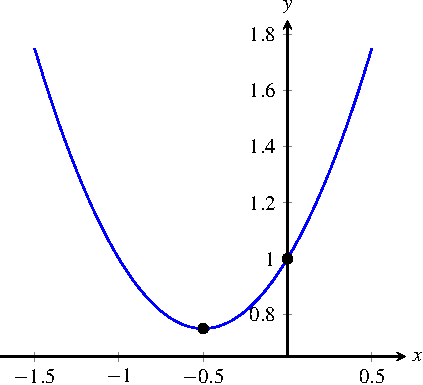
\includegraphics[scale=1]{image/08/a1-b1-c1_vertex-y-intercept.pdf}
\caption{%%
  Graph of the function $f(x) = x^2 + x + 1$ through two points.  The
  two points are the vertex and $y$-intercept of $f(x)$.
}
\label{fig:graph_vertex_y_intercept}
\end{figure}

\solutionpart{subprob:graph_sketch_vertex_y_intercept_fail}
Consider the function $f(x) = x^2$.  The vertex and $y$-intercept of
$f(x)$ are both the same point $\tuple{0}{0}$.  In this case, you have
only one point, not two points required by the above technique for
graph sketching.

\solutionpart{subprob:graph_sketch_vertex_y_intercept_fail_generally}
The function $f(x)$ can be written as
$f(x) = ax^2 + c = ax^2 + 0x + c$.  So $f(x)$ has its vertex at the
$x$-coordinate
%%
\begin{align*}
x
&=
-\frac{0}{2a} \\[4pt]
&=
0.
\end{align*}
%%
The corresponding $y$-coordinate is $y = f(0) = c$.  That is, the
vertex of $f(x)$ is the point $\tuple{0}{c}$.  This point is also the
$y$-intercept of $f(x)$.  If you were to use the above technique for
graph sketching, you would have only one point, not the two required
by the technique.
\end{solution}
}{}

\item Let $w \geq 0$ be a real number.  A rectangle has a width and
  length of $w$ and $4 - w$ centimetres, respectively.  Calculate the
  largest area that the rectangle can have.
\ifbool{showSolution}{
\begin{solution}
Since the width is $w$ and the length is $4 - w$, the area of the
rectangle can be written as the quadratic function
%%
\begin{align*}
f(w)
&=
(4 - w)w \\[4pt]
&=
-w^2 + 4w.
\end{align*}
%%
\Figure{fig:rectangle_largest_area} shows a graph of $f(w)$ to help
you understand how the area $f(w)$ of the rectangle changes as the
width $w$ increases.  From the figure, note that the vertex of $f(w)$
is the highest point in the graph of $f(w)$.  Using
\Expression{eqn:parabola_tip_x_coordinate} the vertex of $f(w)$ occurs
when the width is
%%
\begin{align*}
w
&=
-\frac{4}{2(-1)} \\[4pt]
&=
2.
\end{align*}
%%
The value of $f(w)$ when $w = 2$ is
%%
\begin{align*}
f(2)
&=
2(4 - 2) \\[4pt]
&=
2(2) \\[4pt]
&=
4.
\end{align*}
%%
Conclude that the largest area of the rectangle is $4$ centimetres
squared and this maximum value occurs when the width is $2$
centimetres.

\begin{figure}[!htbp]
\centering
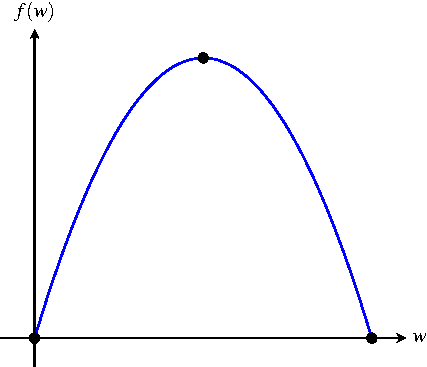
\includegraphics[scale=1]{image/08/rectangle-largest-area.pdf}
\caption{%%
  Graph of the function $f(w) = (4 - w)w$.  Here, $w$ denotes the
  width in centimetres of a rectangle and $f(w)$ represents the area
  in centimetres squared of the rectangle.  Starting from $w = 0$, as
  the width increases the area $f(w)$ also increases up to the highest
  point in the graph.  The area then decreases no matter how much $w$
  increases.  If the point $\tuple{\alpha}{\beta}$ is the vertex of
  $f(w)$, then the largest value of $f(w)$ is $\beta$ and this value
  occurs when $w = \alpha$.
}
\label{fig:rectangle_largest_area}
\end{figure}
\end{solution}
}{}

\item Provide two different proofs that
  $(x - 1)(x - 2) \neq (x + 1)(x + 2)$.
\ifbool{showSolution}{
\begin{solution}
One way is to use the distributive laws to expand both sides of the
expression $(x - 1)(x - 2) \neq (x + 1)(x + 2)$.  Doing so for the
left-hand side results in
%%
\begin{align*}
(x - 1)(x - 2)
&=
x^2 -2x - x + 2 \\[4pt]
&=
x^2 - 3x + 2.
\end{align*}
%%
Now expand the right-hand side of $(x - 1)(x - 2) \neq (x + 1)(x + 2)$
to get
%%
\begin{align*}
(x + 1)(x + 2)
&=
x^2 + 2x + x + 2 \\[4pt]
&=
x^2 + 3x + 2.
\end{align*}
%%
Thus expanding the left- and right-hand sides of the expression
\[
(x - 1)(x - 2)
\neq
(x + 1)(x + 2)
\]
results in two different quadratic functions.

Here is another way to prove that
%%
\begin{equation}
\label{eqn:quadratic_inequality}
(x - 1)(x - 2)
\neq
(x + 1)(x + 2).
\end{equation}
%%
If you have the equality $(x - 1)(x - 2) = (x + 1)(x + 2)$, then the
equality must be true no matter what the value of $x$ is.  However, to
show that the \Inequality{eqn:quadratic_inequality} is true, you need
only provide one value of $x$ such that the left- and right-hand sides
of the expression are different.  Suppose you have $x = 1$.  The
left-hand side of~\eqref{eqn:quadratic_inequality} is
%%
\begin{align*}
(x - 1)(x - 2)
&=
(1 - 1)(1 - 2) \\[4pt]
&=
0(1 - 2) \\[4pt]
&=
0.
\end{align*}
%%
For $x = 1$ the right-hand side of~\eqref{eqn:quadratic_inequality} is
%%
\begin{align*}
(x + 1)(x + 2)
&=
(1 + 1)(1 + 2) \\[4pt]
&=
2(3) \\[4pt]
&=
6.
\end{align*}
%%
In other words, you have shown that both sides
of~\eqref{eqn:quadratic_inequality} are different when $x = 1$.
Therefore \Inequality{eqn:quadratic_inequality} is true.
\end{solution}
}{}

\item Let $x$ and $y$ be real numbers with $x \geq 0$ and $y \geq 0$.
  Suppose $b > 0$ is a fixed number such that $x + y = b$.  Determine
  the maximum value of $xy$.
\ifbool{showSolution}{
\begin{solution}
You know that $x + y = b$.  Solve the last equation for $y$ to get
$y = b - x$ and you can now write the product $xy$ as the quadratic
function
\[
f(x)
=
x(b - x).
\]
Use the distributive laws to write the function $f(x)$ as
$f(x) = -x^2 + bx$.  You know that the vertex of $f(x)$ is the point
at which the value of $f(x)$ is highest or lowest.  The $x$-coordinate
of the vertex of $f(x)$ is
%%
\begin{align*}
x
&=
-\frac{b}{2(-1)} \\[4pt]
&=
\frac{b}{2}
\end{align*}
%%
so the corresponding $y$-coordinate is
%%
\begin{align*}
f(b/2)
&=
\frac{b}{2} \parenthesis*{b - \frac{b}{2}} \\[4pt]
&=
\frac{b}{2} \parenthesis*{\frac{2b}{2} - \frac{b}{2}} \\[4pt]
&=
\frac{b}{2} \parenthesis*{\frac{b}{2}} \\[4pt]
&=
\frac{b^2}{4}.
\end{align*}
%%
Note that $f(b/2) = b^2 / 4$ is positive because you have assumed that
$b > 0$.  Therefore the quadratic function $f(x)$ has a maximum value
of $b^2 / 4$, which occurs when $x = b / 2$.
\end{solution}
}{}

\begin{figure}[!htbp]
\centering
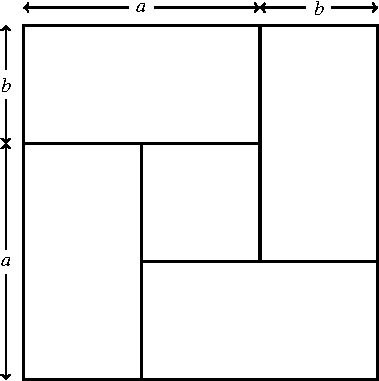
\includegraphics[scale=1]{image/08/arithmetic-geometric-inequality.pdf}
\caption{%%
  A square of side length $a + b$ is divided into four rectangles and
  a smaller square.  Each of the four rectangles has a length and
  width of $a$ and $b$, respectively.
}
\label{fig:arithmetic_mean_geometric_mean_inequality}
\end{figure}

\item Suppose $a \geq 0$ and $b \geq 0$ are fixed numbers.  You will
  prove a special version of an inequality called the
  \emph{arithmetic-mean geometric-mean inequality}.
  %%
  \begin{packedenum}
  \item\label{subprob:AMGM_geometry}
    Let $a + b$ be the side length of a square.  Divide the square
    into smaller shapes as shown in
    \Figure{fig:arithmetic_mean_geometric_mean_inequality}.  Prove
    that
    %%
    \begin{equation}
    \label{eqn:AMGM_geometry}
    4ab
    \leq
    (a + b)^2.
    \end{equation}

  \item\label{subprob:AMGM_inequality}
    Use the result from \Part{subprob:AMGM_geometry} to prove that
    %%
    \begin{equation}
    \label{eqn:AMGM_inequality}
    \sqrt{ab}
    \leq
    \frac{a + b}{2}.
    \end{equation}

  \item\label{subprob:AMGM_equality}
    Determine all values of $a$ and $b$ for which both sides of
    \Expression{eqn:AMGM_inequality} are equal.
  \end{packedenum}
\ifbool{showSolution}{
\begin{solution}
\solutionpart{subprob:AMGM_geometry}
First, you calculate the area of the larger square.  From
\Figure{fig:arithmetic_mean_geometric_mean_inequality} you know that
the larger square has a side length of $a + b$, hence the larger
square has an area of $(a + b)^2$.

Next, you calculate the total area of the four rectangles inside the
larger square.  Each rectangle inside the larger square has a length
and width of $a$ and $b$, respectively, so each rectangle has an area
of $ab$.  Since there are four rectangles inside the larger square, it
follows that the four rectangles have a combined area of
\[
ab + ab + ab + ab
=
4ab.
\]

Finally, you use the areas you calculated above to prove
\Inequality{eqn:AMGM_geometry}.  Let's consider the smaller square at
the centre of the larger square.  You have two cases for the smaller
square:
%%
\begin{packedenumeral}
\item either the smaller square has an area of zero; or

\item the smaller square has an area greater than zero.
\end{packedenumeral}
%%
If the smaller square has an area of zero, then the total area of the
four rectangles is the same as the area of the larger square,
i.e.~$4ab = (a + b)^2$.  If the area of the smaller square is greater
than zero, then the combined area of the four rectangles is smaller
than the area of the larger square, i.e.~$4ab \leq (a + b)^2$.
Therefore no matter what the area of the smaller square is, you will
have the inequality $4ab \leq (a + b)^2$.

\solutionpart{subprob:AMGM_inequality}
From \Part{subprob:AMGM_geometry} you know that $4ab \leq (a + b)^2$.
Since $a + b \geq 0$ because $a \geq 0$ and $b \geq 0$, the square
root of $(a + b)^2$ is the same as $a + b$.  That is, taking the
square root of both sides of the inequality $4ab \leq (a + b)^2$
results in the inequality
\[
\sqrt{4ab}
\leq
a + b.
\]
You know that $\sqrt{4ab} = \sqrt{4} \times \sqrt{ab}$.  Use the fact
that $\sqrt{4} = 2$ to write $2\sqrt{ab} \leq a + b$.  Divide each
side of the latter inequality by $2$ and you have
\[
\sqrt{ab}
\leq
\frac{a + b}{2}
\]
which is the same as \Inequality{eqn:AMGM_inequality}.

\solutionpart{subprob:AMGM_equality}
You have four cases to consider:
%%
\begin{packedenumeral}
\item $a = 0$ and $b = 0$;

\item $a = 0$ and $b > 0$;

\item $a > 0$ and $b = 0$;

\item $a > 0$ and $b > 0$.
\end{packedenumeral}
%%
If $a = 0$ and $b = 0$, then \Inequality{eqn:AMGM_inequality} becomes
\[
\sqrt{0 \times 0}
\leq
\frac{0 + 0}{0}
\]
which simplifies to $0 \leq 0$.  Thus both sides of
\Inequality{eqn:AMGM_inequality} are the same when $a = b = 0$.

If $a = 0$ and $b > 0$, then \Inequality{eqn:AMGM_inequality} can be
written as
\[
\sqrt{0 \times b}
\leq
\frac{0 + b}{2}
\]
which simplifies to $0 \leq \frac{b}{2}$.  Since $b > 0$, then you
have $0 < \frac{b}{2}$.

If $a > 0$ and $b = 0$, then \Inequality{eqn:AMGM_inequality} can be
written as
\[
\sqrt{a \times 0}
\leq
\frac{a + 0}{2}
\]
which simplifies to $0 \leq \frac{a}{2}$.  Since $a > 0$, then you
have $0 < \frac{a}{2}$.  In other words, if exactly one of $a$ and $b$
is zero, then both sides of \Inequality{eqn:AMGM_inequality} are not
the same.

Finally, suppose that $a > 0$ and $b > 0$ and consider again
\Figure{fig:arithmetic_mean_geometric_mean_inequality}.  Note that if
$a = b$, then the area of the smaller square~(at the centre of the
larger square) is zero.  In that case, the area of the larger square
can be written as
\[
(a + b)^2
=
(a + a)^2
=
(2a)^2
=
4a^2.
\]
The length and width of each rectangle are now the same, i.e.~$a$.
Each of the four rectangles has an area of $a^2$.  The total area of
the four rectangles is
\[
a^2 + a^2 + a^2 + a^2
=
4a^2
\]
which is the same as the area of the larger square.  Therefore if
$a = b$, then both sides of \Inequality{eqn:AMGM_inequality} are the
same.
\end{solution}
}{}
\end{problem}

\end{document}
